\section{Architecture of the game}\label{sec:sprint1-architecture}
In this section, we will look at the overall architecture of the different components involved in the game.
\begin{figure}[H]
    \centering
    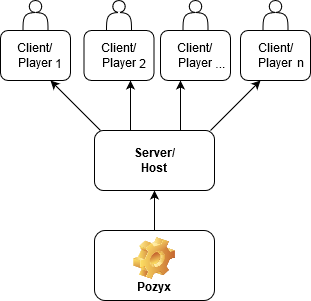
\includegraphics[width=0.6\linewidth]{Architecture.png}
    \caption{The different components of the game}
    \label{fig:architecture}
\end{figure}
\noindent
In \autoref{fig:architecture} an illustration of how we imagine the different components of the game are going to work together is shown.
The arrows in the diagram show the flow of data in the game.
The Pozyx component is responsible for providing the positional data to the host. 
Each client/player is equipped with one of the tags that track their positions on the field. 
The playing field's dimensions will be set to match the distances between the anchors. 
The host has the positional data for each client, but it will also need to know which of the tags each client is equipped with.
The host will then continuously transfer positional data to the clients.
This information will also include which of the tag ids belong to which clients.
Each client will be running an instance of the game, and with the use of the positional data, it will render the playing field, the ball and each of the players.
The host is responsible for checking if the ball has crossed the goal line and it should then provide this information to the players.
In general, the clients' instances of the game should only be responsible for rendering.
Any game logic should happen on the server-side to make sure that the game is synchronized for each player. 
